\begin{activity}{Curie Depth and Magnetic Crustal Thickness}

\section*{Purpose}

This activity explores how temperature limits crustal magnetisation and why deep magnetic structure is long-wavelength.

\section*{Learning Outcomes}

By the end of this activity, you should be able to:
\begin{itemize}
  \item Explain how the Curie temperature limits the depth of crustal magnetisation.
  \item Relate anomaly wavelength to source depth using the depth--wavelength principle.
  \item Compare seismic and magnetic estimates of crustal thickness and explain why they can differ.
  \item Estimate heat flow from Curie depth using a simple geothermal gradient.
\end{itemize}

\begin{questions}
  \question{Curie Depth Concept}
  \begin{enumerate}
    \item What mineral dominates crustal magnetisation?
    \answerbox[1.5cm]
    \item What happens above the Curie temperature?
    \answerbox[2cm]
    \item Is Curie depth a thermal or compositional boundary?
    \answerbox[2cm]
  \end{enumerate}

  \question{Depth and Wavelength}
  Given several magnetic profiles:

  \begin{enumerate}
    \item Which correspond to shallow sources?
    \answerbox[2cm]
    \item Which to deep Curie depth?
    \answerbox[2cm]
    \item How does depth affect short wavelengths?
    \answerbox[2cm]
  \end{enumerate}

  \question{Antarctica Case Study}
  Consider the magnetic and crustal structure of Antarctica (Fig.~\ref{fig:antmag}).
  \begin{figure}[hbt]
      \centering
      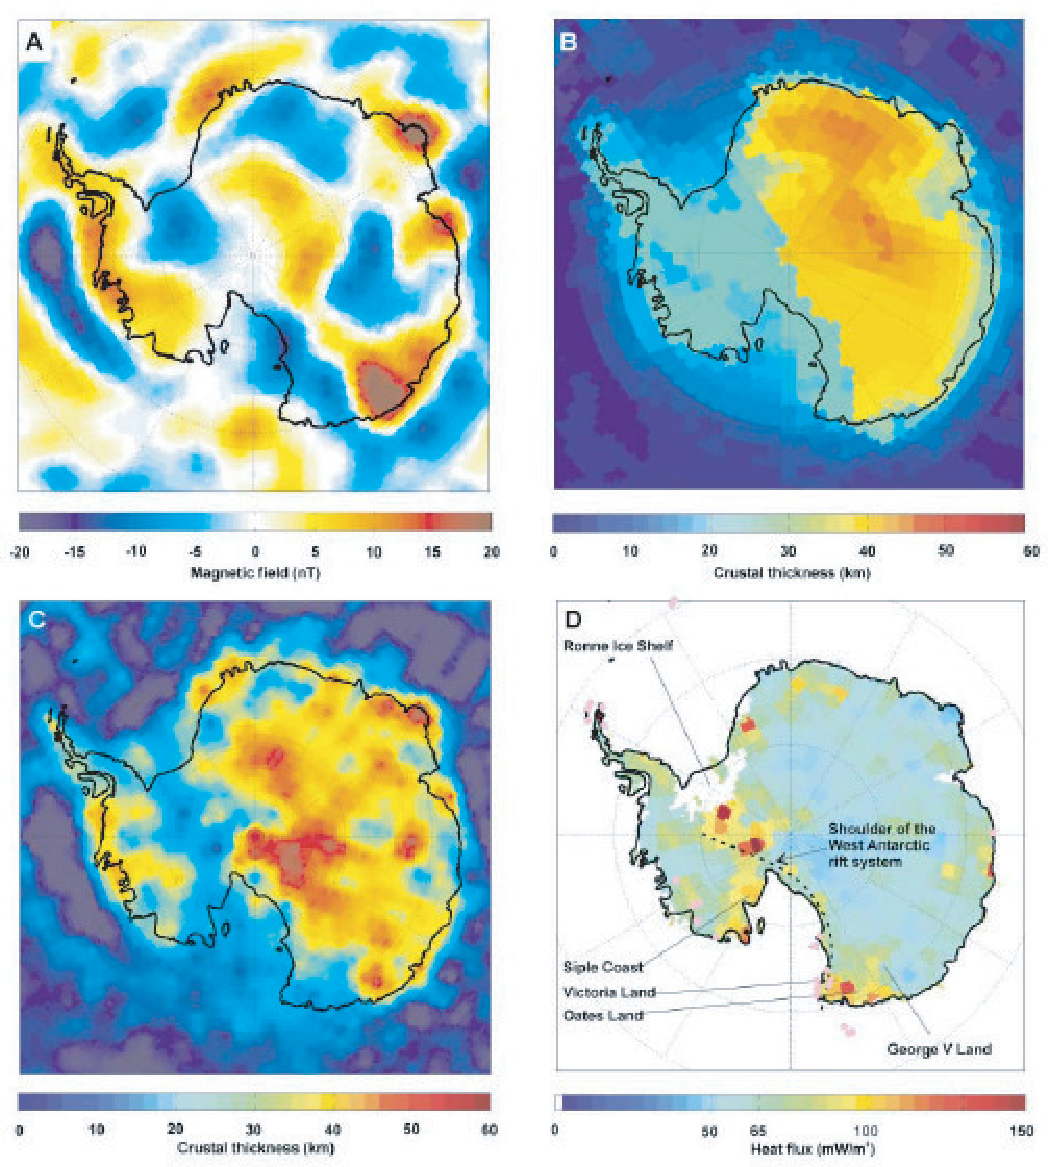
\includegraphics[width=0.75\textwidth]{maule_etal2005.pdf}
      \caption{Estimating the Curie depth from vertical magnetic data.  (a)
      Vertical magnetic field. (b) Crustal thickness model of Antarctica. (c)
      Estimate to base of magnetized layer. (d) Estimated heat flow. Figure
      from Maule et al. ({\bf Science}, 2005).}
      \label{fig:antmag}
  \end{figure}

  Compare:
  \begin{itemize}
    \item Magnetic anomalies
    \item Seismic crustal thickness
    \item Magnetic crustal thickness
  \end{itemize}

  Why do seismic and magnetic thickness estimates differ?
  \answerbox[4cm]

  The first-order geology of Antarctica is characterized by a stable (cratonic) region in East Antarctica and a Cenozoic rift in West Antarctica (Fig.~\ref{fig:antgeo}).
  \begin{figure}[hbt]
      \centering
      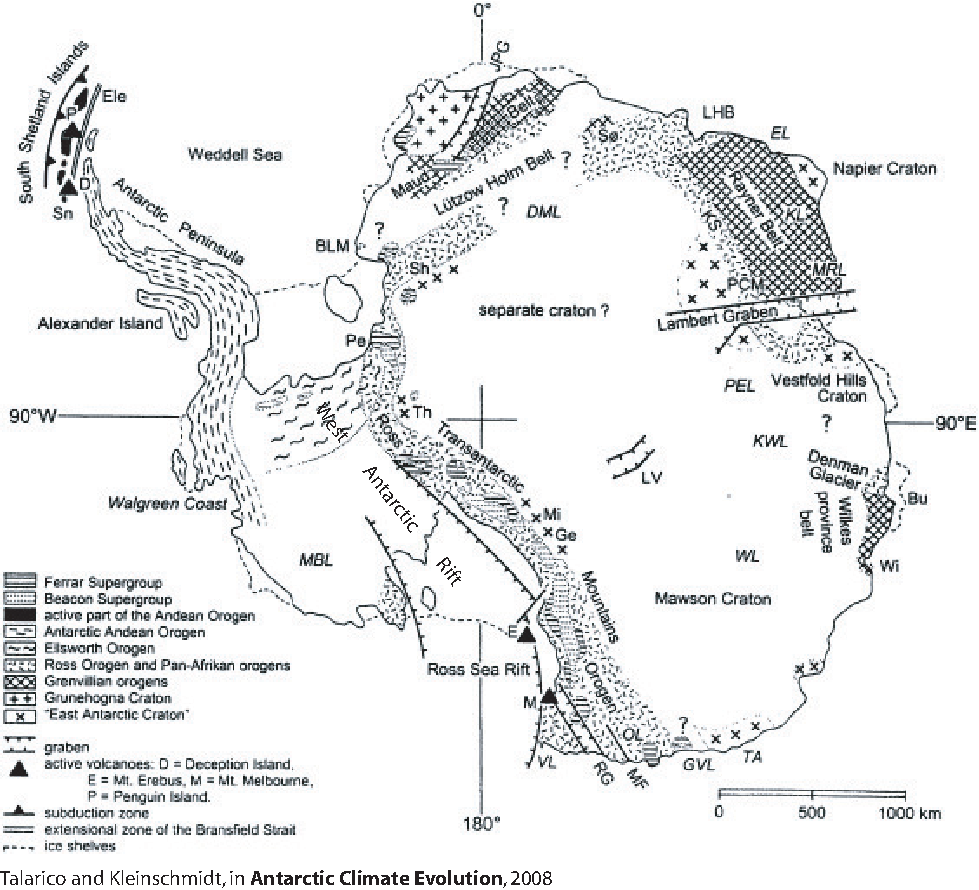
\includegraphics[width=0.75\textwidth]{antarctica_tectonics.pdf}
      \caption{Tectonic map of Antarctica from Talarico and Kleinschmidt ({\bf
      Antarctic Climate Evolution}, 2008).}
      \label{fig:antgeo}
  \end{figure}

  \question{Heat-Flow Estimate}
  The relationship below follows from Fourier's law of steady-state heat
  conduction, assuming a linear temperature increase from the surface to
  the Curie isotherm. We'll discuss this properly when we cover
  conductive heat flow in Week 8 --- for now, take it as given and use it
  to estimate heat flow from the Curie depths you found in Part C.

  Assume:
  \[
    T_C = \SI{570}{^\circ C}, \quad k = \SI{2.8}{W.m^{-1}.K^{-1}}
  \]
  \[
    q = k\frac{T_s - T_C}{z}
  \]
  where $T_s$ is the surface temperature in \si{^\circ C}.

  Estimate heat flow for a rift and a craton.
  \answerbox[5cm]

  \question{Reflection}
  Explain why Curie depth makes magnetics sensitive to thermal structure.
  \answerbox[3cm]
\end{questions}

{\color{red}
\section*{Key Ideas}

\textbf{The Curie temperature defines the base of crustal magnetisation.} Above this temperature (about $580^\circ$C for magnetite), thermal energy prevents the alignment of magnetic domains and the rock is effectively non-magnetic. The depth at which crustal temperatures reach the Curie point therefore sets the maximum depth from which magnetic anomalies can originate.

{\color{blue}
\textbf{Curie depth is a thermal boundary, not a compositional one.} Seismic Moho and magnetic Moho can differ substantially: a hot, thin crust (as in a rift zone) may have its Curie depth within the crust, whereas a cold, thick craton may have Curie depths that approach or exceed the Moho. This is why magnetic thickness and seismic crustal thickness differ systematically between tectonic settings.

\begin{figure}[h]
\centering
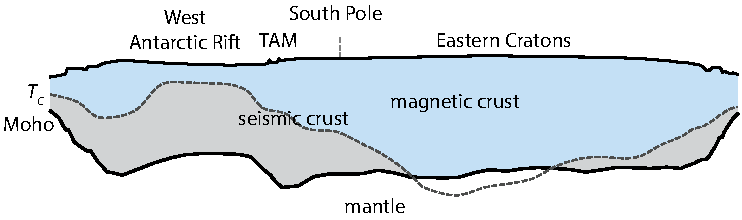
\includegraphics[]{figures/antarctica_profile.pdf}
\caption{The magnetic crustal thickness differs from the seismic crust, which is defined by the depth to the Moho.  The magnetic crustal thickness however is defined by the depth at which rocks are no longer magnetic.  This depth is typically defined by the Curie Isotherm, $T_C$ (approximate closure temperature of magnetite).  There are places where the isotherm dips below the Moho, into the mantle which typically has very low susceptibility.  In such cases, the magnetic crustal thickness is compositionally rather than thermally controlled. While this is a real cross section of crustal thickness and topography of Antarctica, the Curie isotherm is hypothetical.}
\end{figure}
}

\textbf{Curie depth provides a heat-flow estimate.} Assuming a linear geothermal gradient and a known Curie temperature, $q \approx k T_C / z_C$ gives a first-order heat-flow estimate. This is a powerful application because it provides continental-scale heat-flow maps where borehole measurements are unavailable (e.g., beneath Antarctic ice).
}

\end{activity}